\chapter{Passive AC Circuit Analysis}
\label{chap:ACcircuits}
Now that we've covered complex numbers, you are ready to ``dive into'' signal processing! Well, more like ``dip your toes in''. Swimming pool analogy aside, when circuits are designed to manipulate time-varying signals, we use the complex algebra introduced in the last chapter to describe and analyze their behavior. In this chapter, we will learn how.
\section{AC Sources and their Phasor Representations}
AC circuits are driven by AC sources. Those sources are represented in a variety of ways, but the most common representations are shown in Figure \ref{ACsources}. From this figure, we see that the AC voltage symbol is distinct from the DC voltage symbols we have used. However, the AC current symbol is identical to that for DC current sources; context is required to distinguish between AC and DC current sources. 
\begin{figure}[h!]
\centering
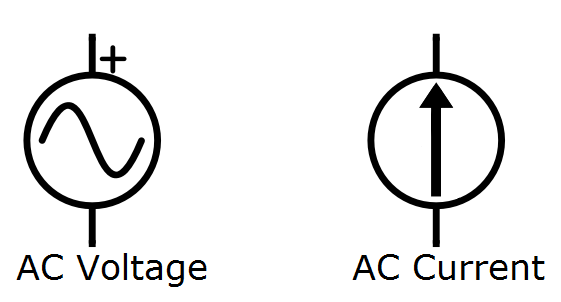
\includegraphics[width=10cm]{figures/ACsources.png}
\caption{Schematic symbols for AC sources. The voltage symbol is clearly different from that for a DC source, but the AC current symbol requires the context of a label to distinguish it from a DC current source.}
\label{ACsources}
\end{figure}
\par
When an AC source is present in a circuit, the time-dependent function of its voltage or current will often be given. When we analyze these circuits, it is always preferrable to do so in phasor notation. This allows us to rely solely on algebra and avoid the unneccesary use of differential equations.\footnote{You might like differential equations. I do, too. However, doing hard things is not what being a professional scientist or engineer is all about. Rather, it's about finding easy ways to do the hard things so you can do them faster! Also, if you take more circuits courses, you will definitely get to practice those DE skills.} So, if you are given a functional description of an AC source, you need to be able to convert that to a phasor representation.
\par
Let's assume we have an AC voltage source that provides a voltage of $V_s(t) = V_0\cos(\omega t + \theta)$. To convert this to phasor form, we need to isolate its magnitude and its phase angle. For this function, like for any cosine function, this is easy; the amplitude is $V_0$, and the phase angle is $\theta$. Therefore, conversion from time-dependent form to phasor form follows this pattern:
$$
V_s(t) = V_0\cos(\omega t + \theta) \leftrightarrow V_0\angle\theta \textnormal{ (with frequency }\omega\textnormal{)}
$$
In addition to the phasor form of our source, its frequency will still be important as we calculate the impedances of the different elements in our circuit; remember that the impedances for both a capacitor and an inductor are dependent on the driving frequency, which will always be the frequency of the AC source in the circuit. 
\par
When we are finished with circuit analysis, we will often want to express our answers in time-dependent form. So, we need to be able to convert a phasor representation into a time-dependent functional representation. To do so only requires us to reverse our steps from before. \textbf{The frequency will not change throughout this process.} 
\section{The Process of AC Circuit Analysis by Example}
Now, let's put all of these equations to work in an example. Most of this will follow what we did in DC.
\begin{figure}[h!]
\centering
\includegraphics[width=10cm]{figures/firstACcircuit.png}
\caption{An AC circuit with an AC voltage source driving a resistor, a capacitor, and an inductor in series.}
\label{myFirstACCircuit}
\end{figure}
\par
Consider the circuit of Figure \ref{myFirstACCircuit}. In this circuit, an AC voltage source is connected to an inductor, a capacitor, and a resistor in series. We need to find the time-dependent voltage across the resistor, $V_R$. To do this, we will rely on the techniques we learned in Chapters \ref{chap:fundamentals} and \ref{chap:resistorRulesAndTricks}, but we will extend them into the realm of complex impedance. But first, we must convert all the quantities given into their equivalent phasor representations.
\par
The voltage source can be represented with the phasor 5V$\angle$0, and we note that its frequency, $\omega$, is 100 rad/s. We will use that frequency to determine the impedances for the inductor and the capacitor according to the expressions for capacitor and inductor impedance from Chapter \ref{chap:capInductorProperties}:
$$
Z_C = \frac{1}{j\omega C} = \frac{1}{j\cdot100\cdot10^{-6}} \Omega= -j\cdot10^{4}\Omega
$$
$$
Z_L = j\omega L = j(100\cdot5) \Omega = j\cdot500\Omega
$$
These impedances are in Cartesian form. Before we proceed, let's also determine their equivalent phasor forms. We can use shortcuts from Chapter \ref{chap:complexAlgebra} in this conversion: $e^{j\pi/2}=j$, and ``$j$''$\rightarrow\angle\pi/2$. Similarly, $e^{-j\pi/2}=-j$, and ``$-j$''$\rightarrow\angle-\pi/2$. Therefore, 
$$
Z_C = -j\cdot10^{4}\Omega = (10^4\angle-\pi/2)\Omega
$$
$$
Z_L = j\cdot500\Omega = (500\angle\pi/2)\Omega
$$
Both of these forms might come in handy, and usually it's a good idea to have both forms available as you begin to analyze a circuit. We should also note that the resistor's impedance has Cartesian and phasor forms, too, but they are simple in comparison with those for the capacitor and inductor because the impedance of the resistor is entirely \textit{real}. Therefore, the Cartesian form for the resistor is just $1000\Omega$, and the phasor form is $(1000\angle0)\Omega$.
\par
Now that we have all the impedances calculated and the phasor representation for the source, we can redraw the circuit using these to label the respective elements, as shown in Figure \ref{myFirstACCircuit2}.
\begin{figure}[h!]
\centering
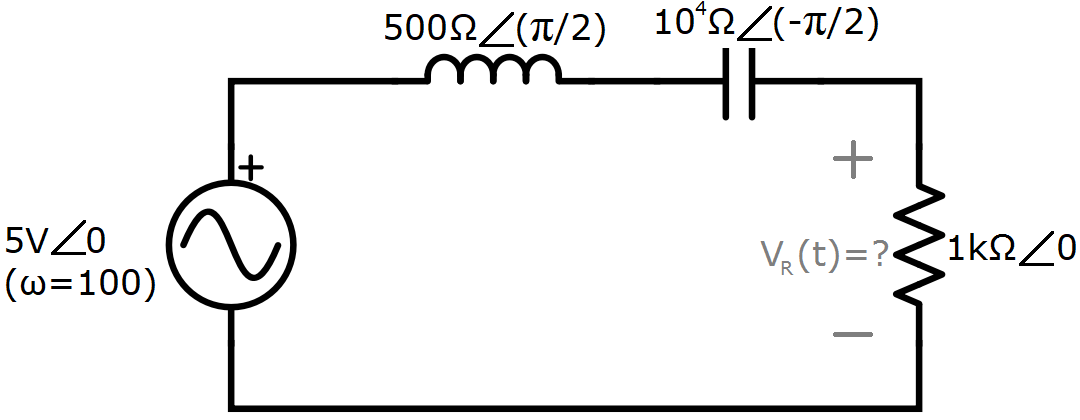
\includegraphics[width=10cm]{figures/firstACCircuit2.png}
\caption{The same circuit as before, but with the elements labeled by the phasor representations of their impedances.}
\label{myFirstACCircuit2}
\end{figure}
 Now that we have calculated the impedances for the capacitor and the inductor, we can use KVL, KCL, Ohm's Law, the Voltage Divider Rule, and the Current Divider Rule to analyze this circuit just like we did for purely resistive DC circuits! This means that if you were able to do the DC analysis in previous chapters, you already have the knowledge required to do what's coming next. 
 \par
 What we want to solve for is the time-dependent voltage across the resistor. In Chapter \ref{chap:resistorRulesAndTricks} we learned that when we have a series of resistances, we can treat those as a \textit{voltage divider}, which allows us to solve for the voltage across one element of the series without having to find the current flowing through that series of elements. This rule extends to complex impedances, which means that we can treat the series of the inductor, capacitor, and resistor as a voltage divider, too, for the purpose of determining the voltage across just the resistor. The total impedance of the series is the sum of their impedances, which is just like the rule we use to combine resistors in series, and  the voltage across the entire series is simply the AC voltage supply. Therefore, the expression for voltage across the resistor is as follows:
 $$
V_R = V_S\cdot\left(\frac{Z_R}{Z_R+Z_C+Z_L}\right)=(5V\angle0)\left(\frac{1000\angle0}{(1000 + j\cdot500 - j\cdot10^4)}\right)
$$
$$
=(5V\angle0)\left(\frac{1000\angle0}{(1000 - j\cdot9500)}\right)
 $$
Before we can finish solving for the phasor form of $V_R$, we need to convert the sum of the three impedances in the denominator from Cartesian form to phasor form. We learned how to do this in Chapter \ref{chap:complexAlgebra}:
$$
1000 - j\cdot9500 = \sqrt{1000^2+9500^2}\angle\arctan(-9500/1000) = 9552.5\angle(-1.46)
$$
Replacing the Cartesian form with this phasor allows us to complete the calculation of the phasor form for $V_R$:
$$
V_R = (5V\angle0)\left(\frac{1000\angle0}{(1000 - j\cdot9500)}\right) = (5V\angle0)\left(\frac{1000\angle0}{9552.5\angle(-1.46)}\right)
$$
$$
= (5V\angle0)\cdot\left(\left(\frac{1000}{9552.5}\right)\angle\left(0- \left(-1.46\right)\right)\right)=(5V\angle0)\cdot(0.1\angle1.46)
$$
$$
=(5\cdot0.1)\angle(0+1.46)=0.5V\angle1.46
$$
With the phasor form for the voltage across the resistor found, we only need to convert that to the time-dependent functional form to be through with this analysis. The amplitude of the voltage is 0.5V, the phase angle is 1.46 radians, and the frequency is the same as the driving frequency, which was 100 rad/s. Putting all these pieces together, we find the functional form for the time-dependent voltage across the resistor: 
$$
v_R(t)= 0.5V\cos(100\cdot t + 1.46)
$$
And that concludes our analysis!
\par
The equations we used in this example were exactly what we would have used if we only had resistors in our circuit; all the rules and tricks we used were the same, except that we were using complex impedance instead of all-real resistance. In other words, the most challenging part about AC circuit analysis as compared to DC circuit analysis is the fact that we are working with complex numbers instead of all real numbers. 
\section{Frequency-Dependent Behavior in AC Circuits}
Now that we are dealing with frequency-dependent impedances, we should examine the effects of changing our source frequency on the results of our calculations. Let's consider the example of the previous section, but let's change the source frequency from 100 rad/s to 10rad/s. Eventually, you will be able to predict the effect of such a frequency change on the voltage across the resistor, but for now, let's recalculate it.
\par
First, we need to calculate the new impedances for the inductor and capacitor. Since the source frequency is now $1/10^{th}$ its previous value, we can adjust the impedances of the inductor and the capacitor by dividing by 10 and multiplying by 10, respectively:
$$
Z_L = j\cdot50\Omega
$$
$$
Z_C = -j\cdot10^5\Omega
$$
Using these values in the above calculation of $v_R(t)$ yields the following result:
$$
V_R = (5V\angle0)\left(\frac{1000\angle0}{(1000 - j\cdot99950)}\right) = (5V\angle0)\left(\frac{1000\angle0}{99955.0\angle(-1.56)}\right)
$$
$$
= (5V\angle0)\cdot\left(\left(\frac{1000}{99955.0}\right)\angle(0- (-1.56))\right) = (5V\angle0)\cdot(0.01\angle1.56)
$$
$$
V_R=0.05V\angle1.56
$$
Therefore,
$$
v_R(t)=0.05V\cos(10\cdot t + 1.56)
$$
\par
From this result, we see that as the source frequency decreases, the amplitude of the voltage drop across the resistor decreases, too. Furthermore, the phase difference across the resistor appears to approach $\pi/2$ as the driving frequency decreases.\footnote{This makes sense, because the dominant impedance of the three passive elements in the circuit is that of the capacitor (by a LOT!), which itself has a phase angle of $-\pi/2$. This phase angle for the capacitor must be compensated for by the phases of the voltages across the resistor and the inductor. Of those two choices, the magnitude of the resistor's impedance is 20$\times$ that of the inductor's impedance, so the majority of the phase must be accounted for across the resistor.}
\par
Now let's see what happens if we \textit{increase} the source frequency of the example circuit from the previous section from 100rad/s to 1000rad/s. I will leave out the majority of the steps here:
$$
V_R = (5V\angle0)\cdot\left({1000}{1000+j\cdot4000}\right) = (5V\angle0)\cdot(0.24\angle1.33)
$$
$$
V_R = 1.2V\angle1.33
$$
Therefore,
$$
v_R(t) = 1.2V\cos(1000\cdot t +1.33)
$$
Compared to the initial result from the previous section, the amplitude of the voltage across the resistor has more than doubled, and the phase has decreased. Of course, if we increase the frequency indefinitely, the impedance of the inductor will increase, too, eventually dominating the total impedance of the series of elements. From this, we can see that the choice of source frequency has a dramatic impact on the results of AC circuit analysis. Let's make one more change and see what the result is.
\par 
During the last round of calculation, we saw a change in the sign of the imaginary part (which we refer to as the \textit{reactance}) of the total impedance of the series of elements. This happened because the impedance of the inductor became greater in amplitude than that of the capacitor, and those two quantities work against each other in the total calculation. Let's determine 1) what source frequency causes those two impedances to cancel each other out, and 2) what the $v_R$ is in that case.
\par
First, if we set $Z_L+Z_C=0$, we can solve for $\omega$ in that case:
$$
j\cdot5\omega -j\cdot\frac{1}{\omega10^{-6}}= 0
$$
$$
5\omega = \frac{1}{10^{-6}\omega}
$$
$$
\omega^{2} = \frac{1}{5\cdot10^{-6}} \textnormal{ rad$^2$/s$^2$}
$$
$$
\omega = \sqrt{\frac{1}{5\cdot10^{-6}}}\textnormal{ rad/s} = 447.21 \textnormal{ rad/s}
$$
This frequency is referred to as the \textit{resonant} frequency for the circuit because it causes the inductor and capacitor impedances to resonate with each other, canceling each other out in the process. 
\par
Now that the resonant frequency has been determined, let's set the source frequency to the resonant frequency and calculate $v_R(t)$ again:
$$
V_R = (5V\angle0)\cdot\left(\frac{1000\angle0}{1000 + j\cdot\cancel{(2236.05 - 2236.05)}}\right)
$$
$$
V_R = 5V\angle0
$$
Therefore,
$$
v_R(t) = 5V\cos(1000\cdot t) = v_s(t)
$$
In this case, the voltage across the resistor is exactly the same as the supply voltage! This may seem crazy, but if you calculate the voltages across the capacitor and the inductor in this case, you will see that they are equal to each other in amplitude but opposite each other in phase. Therefore, they experience perfect destructive interference. Aren't waves cool?
\par
Hopefully this exercise has shown you that 1) the frequency dependence of AC circuits brings about some weird and interesting behavior, and 2) we didn't need to learn a lot of new stuff to do this analysis. In the next chapter, we will take a more applied look at frequency dependence in AC circuits and how it can be used to accomplish the useful task of filtering a signal.
\section{Recap: Passive AC Circuits}
Hopefully this chapter built up your confidence in your knowledge of circuit analysis. Gaining comfort with complex numbers is the main challenge with AC analysis, but all the rules for DC analysis still apply.
\begin{description}
\item[Converting Time-Dependent Sources to Phasor Notation:] When the time-dependent function for a source is given, that source can be represented in phasor form by the following conversion, and the conversion can be carried out in both directions:
$$
V_s(t) = V_0\cos(\omega t + \theta) \leftrightarrow V_0\angle\theta \textnormal{ (with frequency }\omega\textnormal{)}
$$
\end{description}
